\documentclass[11pt,letter]{exam}
\usepackage{listings}
\usepackage{tabularx}

\newif\ifpdf
\ifx\pdfoutput\undefined
\pdffalse % we are not running PDFLaTeX
\else
\pdfoutput=1 % we are running PDFLaTeX
\pdftrue
\fi

\ifpdf
\usepackage{subfigure}
\usepackage[pdftex]{graphicx}
\else
\usepackage{graphicx}
\fi

\firstpageheader{\bf\Large CS 151}{\bf\Large Final Exam}{\bf\Large
  May 18, 2004}
\runningheader{CS 151}{}{Exam-2}
\addpoints

\begin{document}

\begin{center} 
  \fbox{\fbox{\parbox{5.5in}{\centering This Quiz is being given under
        the guidelines of the \textbf{Honor Code}. You are expected to
        respect those guidelines and to report those who do not.
        Answer the questions in the spaces provided. If you run out of
        room for an answer, continue on the back of the page.  There are
      \numquestions\  questions for a total of  \numpoints\ points.}}}
\end{center} 
\lstset{language=Java,numbers=left}

\vspace{0.1in} 
\hbox to \textwidth{Name:\enspace\hrulefill} 


\begin{questions}

% Some unix commands....
\question[5]
Bob Memoryleak has forgotten where he saved the file for his latest computer
science homework.  He recalls that He named the class BinTree, and that the file
is in some subdirectory under his home.  What command 
could Bob use to find the file.
\vspace{0.5in}

\question[5]
Once again our forgetful friend Bob has gotten himself into trouble. He has been
writing all of his Paidea papers in emacs and saving them as text files. His
directory of term papers has many files in it including files named like
blah.txt, foobar.txt, longone.txt, and others. He's searching for the paper he
wrote on the importance of Oooblech in the medieval feudal system. What command
could Bob use to locate the paper he is looking for?
\vspace{0.5in}
% Algorithmic Analysis

\question[10]
The following table shows running times for a set of algorithms that solve:
a problem of teh size given in the left column.  Fill in the next two rows: 
\begin{table}[h]
  \centering
  \begin{tabularx}{5in}{|r|X|X|X|X|X|}
    \hline
     $N$ & $O(N^3)$ & $O(N^2)$ & $O(N log{N})$ &  $O(N)$ & $O(1)$ \\[10pt]
    \hline
    10 &  100 &  10 & 8 &  1 & 5 \\[10pt]
    \hline
    100 &  &  &  &  &  \\[10pt]
    \hline
    10,000 &  &  &  &  &  \\[10pt]
    \hline
  \end{tabularx}

\end{table}
\newpage
\question[20]
A palindrome is a word (or phrase) that reads the same both forward and
backward. We can ignore punctuation marks and white space. Palindromes have been around since biblical
times. For example, when Adam and Eve first met Adam is quoted as saying ``madam I'm adam''.
Later in history a large engineering feat in central america was described as:
``a man a plan a canal panama''. When the use of electricty became widespread,
engineers were often heard muttering ``so many dynamos''. Write a recursive
function \texttt{boolean pal(String s)} to dermine whether a given string is a
palindrome. For example: \texttt{pal(palprep("go hang a salami! I'm a lasagna hog"))} 
would return true, whereas \texttt{pal("palindrome")} would return false.  
You do not need to write the palprep method. It simply returns a string with 
punctuation and spaces removed.  \textit{Hint: a zero or one character string is always
a palindrome, a two character string is a palindrom if the two characters are
the same...}


\newpage
\question[10] Using the \textit{Median of 3} approach, show each step
in the quicksort paritioning process as quicksort processes the following array
of numbers.  When you are done make sure that you clearly identify $L$, $R$, and
the pivot. 
\begin{figure}[h]
  \centering
  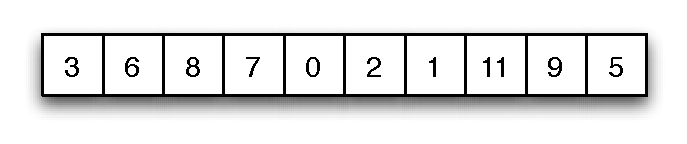
\includegraphics{part-array.pdf}
\end{figure}

\newpage
\question[20]
The following graph shows the closest websites that link between themselves and
the uther college computer science homepage.  Show two different data structures for
representing the graph.
\begin{figure}[h]
  \centering
  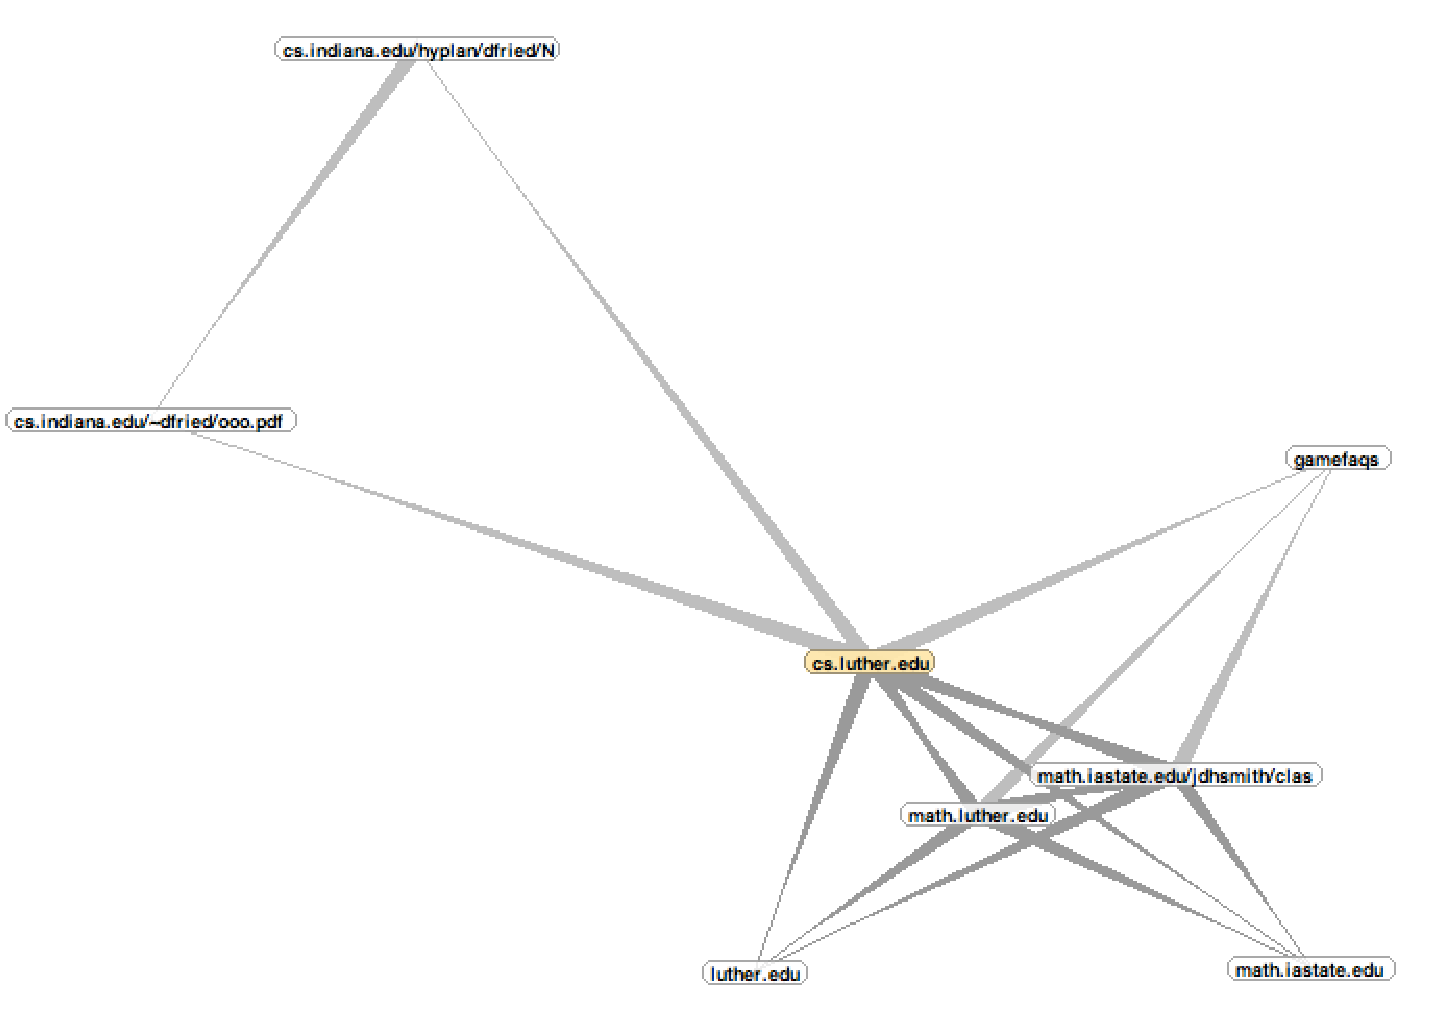
\includegraphics[height=4.5in]{cs-graph.pdf}
\end{figure}

\newpage
\question
Optical cable used in networking can be extremely expensive: hundreds of dollars
per meter. Whoever is paying for that is going to want to use the least amount
possible. Suppose we have to wire an entire college campus with this to give
incoming freshmen terabit ethernet capabilities. There are hundreds if not
thousands of ways we could choose to run the wires between buildings. We want to
find the best without examining the cost of every possibility.  We can use the
minimal spanning tree algorithm to solve this problem.  The following table
shows the connections from the building in the first column to the building in
the second column, with the weight provided in the third column.
\begin{verbatim}
1 2 10
1 3 15
1 6 25
1 10 11
2 3 7
3 4 7
3 6 10
4 5 7
4 6 5
5 6 13
5 7 17
6 10 15
6 9 10
6 7 6
6 8 10
7 8 7
8 9 6
9 10 10
\end{verbatim}
\begin{parts}
\part[10]
Draw the directed graph represented by the above table.
\part[10]
Show the minimal spanning tree constructed from the graph using kruskals algorithm.  
You must show the edges that are in the spanning tree at each step of the
algorithm so that I know you understand how the algorithm works.

\end{parts}

\newpage
\question[10]
Given the following insert operations into a hash table that uses linear
probing, and the hash function $h(x) = x * 11 \% 20 $  Show the keys stored at
each position of the hash key array.
insert(10)
insert(20)
insert(40)
insert(111)
insert(15)
insert(11)
insert(110)
insert(45)
\begin{figure}[h]
  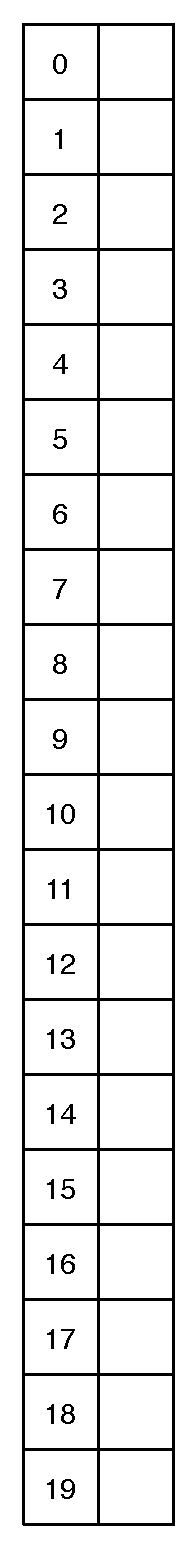
\includegraphics[height=6.5in]{HashTab.pdf}
\end{figure}
\newpage
\question[20]
% Perform a topological sort on the following graph.
The classes that need to be taken in order to get a computer science major can
be represented as a graph.  Part of the graph for a CS major is shown in figure
\ref{fig:cs}
\begin{figure}[ht]
  \label{fig:cs}
  \centering
  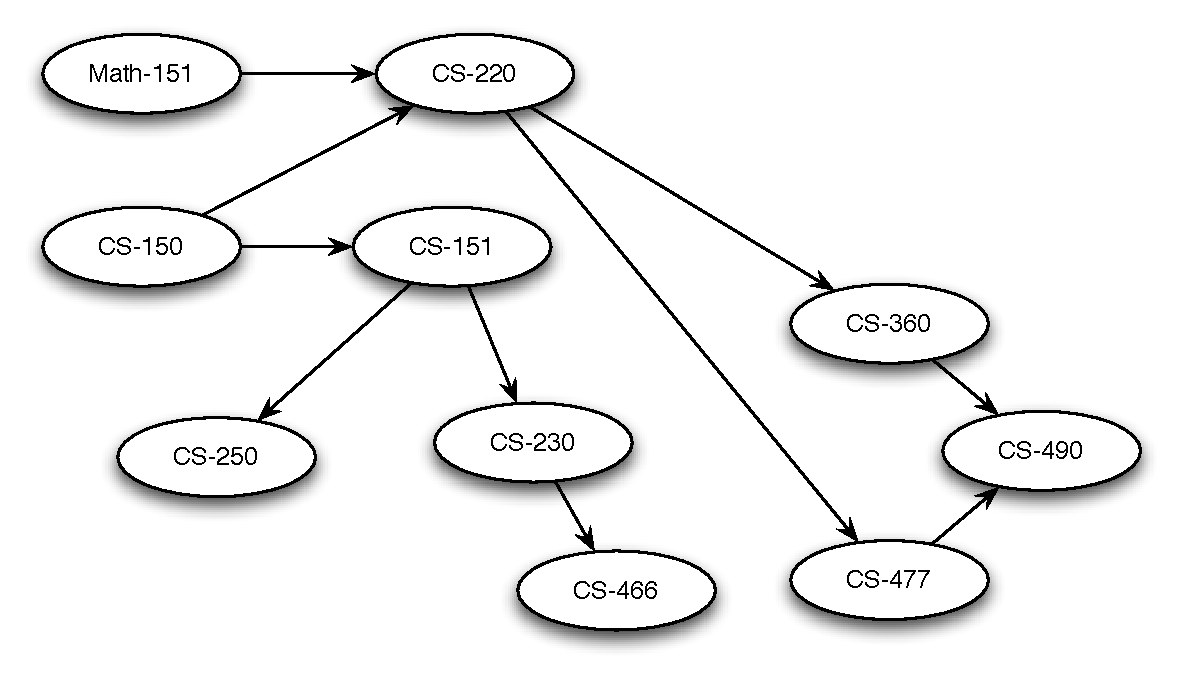
\includegraphics[height=2.5in]{prereq-graph.pdf}
\end{figure}
Although the prerequisites may seem complicated at first, a topological sort can
help you plan your schedule for the coming years.  Show the result of running
the topological sort algorithm on the graph of classes required for the CS major.  

\newpage
\question[20]
Assume that you have a LinkedList class just like the one we built in class.
That is you have a LinkedList class with a head node, and a LinkNode class.
defined as follows: 
\begin{lstlisting}
class LinkNode {
    Comparable payload
    LinkNode next
}
\end{lstlisting}
We can create a new class called SortedLinkedList by extending the LinkedList 
class and overloading the add(Object) method to be add(Comparable).  The new add
method must insert the new object in the list in such a way that the list is in
sorted order.  Write the java code for this new add method.

\newpage
\question[20]
Assume that you have A BinaryHeap class with the following methods:
\begin{itemize}
\item BinaryHeap()  -- Constructor
\item void insert(Comparable)  -- add an element to the heap
\item Comparable delMin()  -- remove the smallest element from the heap
\item void buildHeap(Comparable []). -- initialize a heap from an array
\end{itemize}
Using the BinaryHeap class, write the code to implement a sort algorithm:
Comparable[] heapSort(Comparable []).  
What is the running time of the algorithm? Justify your answer.

% Write a level-order traversal for a binary tree (using a queue).

\end{questions}

\end{document}

